% !TEX root = CW_UL_1.tex

\documentclass[10pt,a4paper]{article}

\usepackage[a4paper,top=1.8cm,bottom=1.8cm,left=2.0cm,right=2.0cm]{geometry}
\usepackage{amsmath,amssymb}
\usepackage{graphicx}
\usepackage{booktabs}
\usepackage{xcolor}
\usepackage{listings}
\usepackage{float}
\usepackage{caption}
\usepackage{enumitem}
\usepackage[colorlinks=true,allcolors=blue]{hyperref}

\captionsetup{font=small,labelfont=bf}

% --- Python listing style ---
\definecolor{kw}{rgb}{0.13,0.13,0.6}
\definecolor{str}{rgb}{0.6,0.13,0.13}
\definecolor{cmt}{rgb}{0.35,0.45,0.35}
\lstdefinestyle{py}{
  language=Python,
  basicstyle=\ttfamily\scriptsize,
  keywordstyle=\color{kw}\bfseries,
  stringstyle=\color{str},
  commentstyle=\color{cmt}\itshape,
  showstringspaces=false,
  breaklines=true,
  columns=fullflexible,
  keepspaces=true,
  frame=single,
  framesep=4pt,
  rulecolor=\color{gray!40},
  aboveskip=4pt,belowskip=4pt,
}
\lstset{style=py}

\setlength{\parskip}{2pt}
\setlength{\parindent}{0pt}

\title{\vspace{-1.2cm}\textbf{MATH70102 Unsupervised Learning --- Coursework 1}}
\author{}
\date{}

\begin{document}
\maketitle
\vspace{-1.0cm}

\section*{Generative AI Usage}

\textbf{NotebookLM} (Google) was used to query and cross-reference the course lecture notes and slides, helping identify the correct algorithmic approach for each problem (e.g.\ confirming the appropriate NMF update rule and the SMACOF convergence settings for MDS). \textbf{Claude} (Anthropic) was used to assist with typesetting this \LaTeX{} document. All analysis, code, mathematical derivations, and written answers are the author's own work.

% ============================================================
\section{Denoising the Egyptian Goose with PCA and NMF}

\subsection{Problem and approach}

We are given a clean and a noisy $512\times512$ greyscale image of an Egyptian goose, as pixel matrices $X_{\text{clean}}$ and $X_{\text{noisy}}$. For a selection of integers $q$ covering $1,\dots,512$ we reconstruct the noisy image in two ways and measure how close each reconstruction is to the clean image in \emph{Euclidean (Frobenius) distance}
\[
  d(A,B)=\sqrt{\textstyle\sum_{i,j}(A_{ij}-B_{ij})^2}.
\]
\textbf{PCA} (Week~2): treating the $512$ rows as samples in $\mathbb{R}^{512}$, we keep the first $q$ principal components and reconstruct. \textbf{NMF} (Week~3): we factorise $X_{\text{noisy}}\approx WH$ with $W\in\mathbb{R}^{512\times q}_{\ge 0}$, $H\in\mathbb{R}^{q\times 512}_{\ge 0}$ and reconstruct via $WH$. Writing $d_0=d(X_{\text{clean}},X_{\text{noisy}})$ for the baseline, a method \emph{denoises} if some $q$ gives $d(X_{\text{clean}},\hat X_q)<d_0$.

We load the data and define the distance. The noisy image is already strictly positive, so it is directly admissible to NMF without the $+1.01$ shift used in the Week~3 digit example (whose data lived in $[-1,1]$ with zeros).

\begin{lstlisting}
import matplotlib.pyplot as plt
import numpy as np
import numpy.typing as npt
from sklearn.decomposition import PCA

X_clean = np.loadtxt("egyptian_goose_clean.csv", delimiter=",")
X_noisy = np.loadtxt("egyptian_goose_noisy.csv", delimiter=",")

def euclid(A, B):                       # Euclidean / Frobenius distance
    return np.sqrt(np.sum((A - B) ** 2))

baseline = euclid(X_clean, X_noisy)     # d_0 = 29.5459
\end{lstlisting}

\subsection{Choosing the grid of \texorpdfstring{$q$}{q} via a scree plot}

We let the data guide the grid using a scree plot of the noisy image's principal components --- the Week~2 tool for deciding how many components to retain. The variance is heavily front-loaded (PC1 alone $\approx27\%$, PC2 $\approx14\%$; $80\%$ is reached at $q=42$, $95\%$ at $q=188$), so we sample densely at low $q$, refine over the mid-band where most variance is captured, and keep a coarse tail to $q=512$ (included as a check: there the reconstruction must equal the noisy image).

\begin{lstlisting}
scree = PCA().fit(X_noisy)
evr = scree.explained_variance_ratio_
cum = np.cumsum(evr)

fig, axs = plt.subplots(1, 2, figsize=(8, 2.7))
axs[0].bar(range(1, 31), evr[:30] * 100, color="salmon")
axs[0].set_xlabel("Principal component"); axs[0].set_ylabel("Explained variance (%)")
axs[1].plot(range(1, len(cum) + 1), cum * 100, color="royalblue")
axs[1].set_xlabel("Number of components q"); axs[1].set_ylabel("Cumulative (%)")

q_grid = np.array(sorted(set(
    list(range(1, 21))
    + [25, 30, 35, 40, 45, 50, 55, 60, 65, 70, 75, 80, 90, 100]
    + [110, 125, 150, 175, 200, 225, 250, 275, 300]
    + [350, 400, 450, 500, 512])))
\end{lstlisting}

\begin{figure}[H]
  \centering
  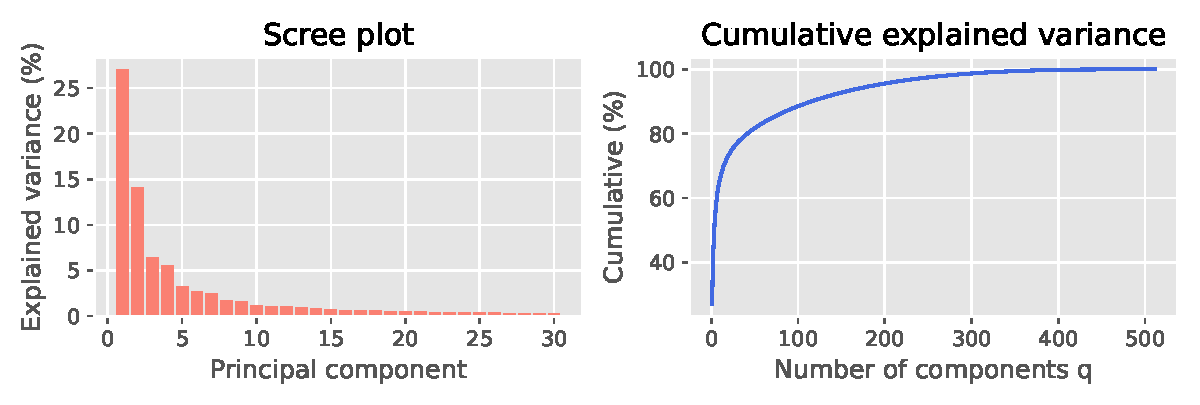
\includegraphics[width=0.86\textwidth]{fig_scree.pdf}
  \caption{Scree plot (left) and cumulative explained variance (right) of the noisy image. The steep decay justifies dense sampling at low $q$.}
\end{figure}

\subsection{PCA reconstruction (Week 2)}

For each $q$ we fit \texttt{PCA(n\_components=q)}, project with \texttt{fit\_transform}, and reconstruct with \texttt{inverse\_transform}. PCA re-adds the sample mean, so at $q=512$ the noisy image is recovered exactly.

\begin{lstlisting}
pca_dist = np.empty(len(q_grid)); pca_recons = {}
for i, q in enumerate(q_grid):
    pca = PCA(n_components=int(q))
    recon = pca.inverse_transform(pca.fit_transform(X_noisy))
    pca_dist[i] = euclid(X_clean, recon)
    pca_recons[int(q)] = recon

best_pca_idx = int(np.argmin(pca_dist)); best_pca_q = int(q_grid[best_pca_idx])
# PCA: best q = 80 -> d = 24.9536;  d at q=512 = 29.5459 (= baseline)
\end{lstlisting}

\subsection{NMF reconstruction (Week 3)}

We use the \texttt{NMF\_numpy} class from the Week~3 reference \emph{verbatim}. It maximises the quasi-likelihood $L(W,H)=\sum X\odot\log(WH)-WH$ by multiplicative updates; the reconstruction is stored in \texttt{.WH}.

\begin{lstlisting}
class NMF_numpy:
    def train(self, X: npt.NDArray[np.number], q: int, n_iter: int = 100) -> None:
        d, n = X.shape
        self.W = np.random.uniform(low=0, high=1, size=(d, q)).astype(X.dtype)
        self.H = np.random.uniform(low=0, high=1 / q, size=(q, n)).astype(X.dtype)
        self.WH = self.W @ self.H
        self.logL = np.empty(n_iter, dtype=X.dtype)
        self.dist = np.empty(n_iter, dtype=X.dtype)
        for a in range(n_iter):
            self.W *= ((X / self.WH) @ self.H.T) / self.H.sum(axis=1)[None, :]
            self.WH = self.W @ self.H
            self.H *= (self.W.T @ (X / self.WH)) / self.W.sum(axis=0)[:, None]
            self.WH = self.W @ self.H
            self.logL[a] = np.sum(X * np.log(self.WH) - self.WH)
            self.dist[a] = np.sum((X - self.WH) ** 2)
\end{lstlisting}

A convergence check at $q=20$ (Figure~\ref{fig:conv}) shows the objective flattens well before 500 iterations, so we use \texttt{n\_iter\,=\,400} in the sweep, with the random $W,H$ initialisation seeded for reproducibility.

\begin{lstlisting}
np.random.seed(0)
check = NMF_numpy(); check.train(X_noisy, q=20, n_iter=500)
fig, axs = plt.subplots(1, 2, figsize=(8, 2.4))
axs[0].plot(range(1, 501), check.logL, color="red");  axs[0].set_ylabel(r"$L(W,H)$")
axs[1].plot(range(1, 501), check.dist, color="blue"); axs[1].set_ylabel(r"$\|X-WH\|^2$")

np.random.seed(0)
nmf_dist = np.empty(len(q_grid)); nmf_recons = {}
for i, q in enumerate(q_grid):
    nmf = NMF_numpy(); nmf.train(X_noisy, int(q), n_iter=400)
    nmf_dist[i] = euclid(X_clean, nmf.WH)
    nmf_recons[int(q)] = nmf.WH

best_nmf_idx = int(np.argmin(nmf_dist)); best_nmf_q = int(q_grid[best_nmf_idx])
# NMF: best q = 275 -> d = 25.2179
\end{lstlisting}

\begin{figure}[H]
  \centering
  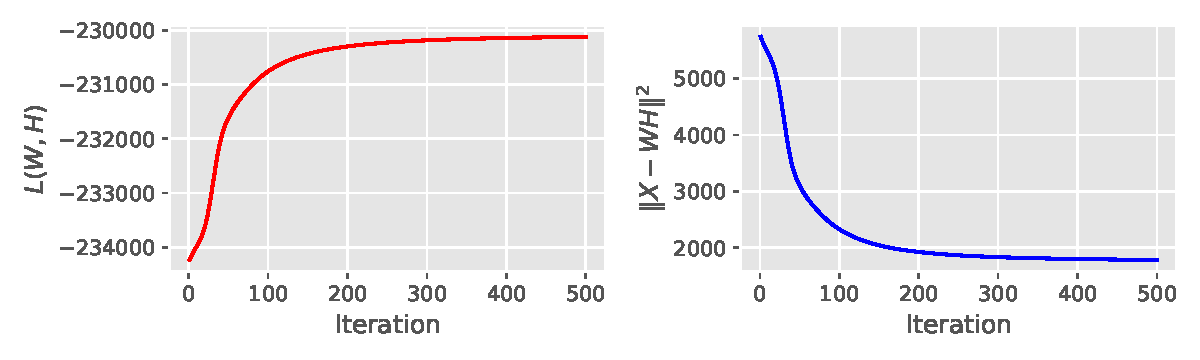
\includegraphics[width=0.72\textwidth]{fig_conv.pdf}
  \caption{NMF convergence at $q=20$: quasi-likelihood $L(W,H)$ (left) and reconstruction error $\|X-WH\|^2$ (right) against iteration. Both have plateaued by $\sim$200 iterations.}
  \label{fig:conv}
\end{figure}

\subsection{Results}

\begin{lstlisting}
plt.plot(q_grid, pca_dist, "-o", label="PCA")
plt.plot(q_grid, nmf_dist, "-s", label="NMF")
plt.axhline(baseline, linestyle="--", label="Baseline = %.2f" % baseline)
plt.xlabel("q"); plt.ylabel("distance to clean image"); plt.legend()
\end{lstlisting}

\begin{table}[h]
  \centering\small
  \begin{tabular}{lccccc}
    \toprule
     & best $q$ & $d(X_{\text{clean}},\hat X_q)$ & improvement vs.\ $d_0$ & cum.\ variance at $q$ & denoises? \\
    \midrule
    Baseline (noisy) & --- & $29.55$ & --- & --- & --- \\
    PCA & $80$  & $24.95$ & $4.59$ & $86\%$ & \textbf{yes} \\
    NMF & $275$ & $25.22$ & $4.33$ & $98\%$ & \textbf{yes} \\
    \bottomrule
  \end{tabular}
  \caption{Best reconstructions. PCA beats the baseline for all $q\in[25,500]$; NMF for all $q\in[35,512]$.}
\end{table}

\begin{figure}[H]
  \centering
  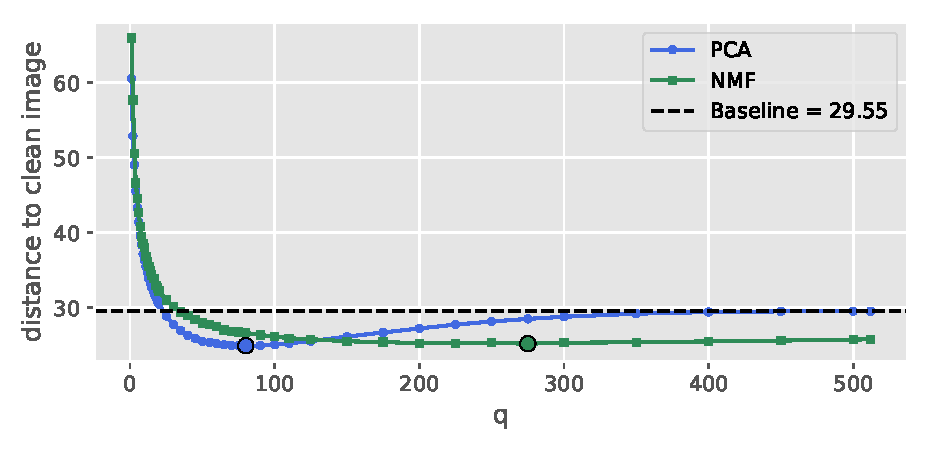
\includegraphics[width=0.90\textwidth]{fig_curve.pdf}\\[2pt]
  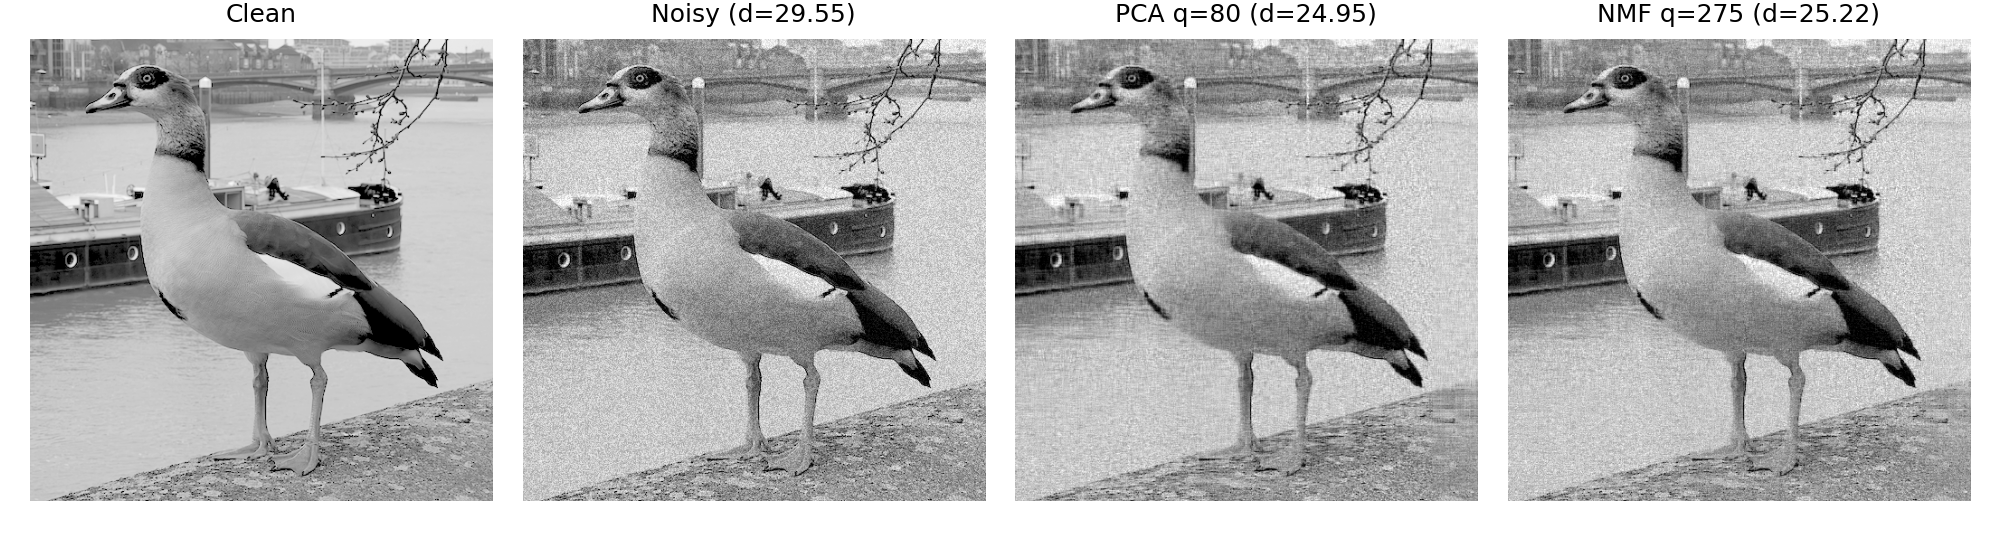
\includegraphics[width=0.99\textwidth]{fig_compare.png}
  \caption{Top: distance to the clean image versus $q$; both curves dip well below the baseline (dashed) and the marked points are the optima. Bottom: clean, noisy, and best-$q$ PCA/NMF reconstructions (displayed on the clean image's intensity range).}
\end{figure}

\subsection{Conclusion}

\textbf{Yes --- both PCA and NMF denoise the image.} For each method there is a wide band of $q$ giving a reconstruction strictly closer to the clean image than the noisy image is: the distance falls from $d_0=29.55$ to $24.95$ (PCA, $q\approx80$) and $25.22$ (NMF, $q\approx275$). The distance-versus-$q$ curve is \textbf{U-shaped}. Noise spreads its energy across all $512$ directions, whereas the image's structure is concentrated in the leading components (scree plot: PC1 $\approx27\%$). For small $q$ the reconstruction under-fits and discards genuine structure; at an intermediate $q$ it keeps the signal while rejecting the many noise-dominated high-index components --- the denoising optimum; and as $q\to512$ it recovers the noisy image ever more faithfully, so the distance climbs back to $d_0$ (for PCA this is exact, verified at $q=512$). PCA reaches its optimum earlier and slightly lower than NMF, consistent with its components being the variance-optimal directions, so it concentrates the signal into fewer of them. The improvement is real but moderate ($\approx15\%$): broadband noise can only be partly removed by a low-rank truncation, since only the portion of the noise lying in the discarded components is rejected.

% ============================================================
\section{Mapping Airports with Multidimensional Scaling}

\subsection{Problem and approach}

We are given great-circle distances (km) between six northern-hemisphere airports (Table~\ref{tab:airports}). The task is to \emph{draw a map} --- an embedding in $\mathbb{R}^2$ that reproduces these distances as faithfully as possible in relative terms. This is exactly the setting for \textbf{multidimensional scaling (MDS)} (Week~4): given only pairwise dissimilarities $d_{ij}$, MDS places points $z_1,\dots,z_n$ in $\mathbb{R}^q$ to minimise the \emph{least-squares stress}
\[
  S_M(z_1,\dots,z_n) = \sum_{i\neq j}\bigl(d_{ij} - \lVert z_i - z_j\rVert\bigr)^2.
\]
We use \texttt{sklearn.manifold.MDS} with \texttt{dissimilarity="precomputed"}, following the Week~4 reference solution.

\begin{table}[h]
  \centering\small
  \begin{tabular}{lrrrrr}
    \toprule
           & CPH   & EWR    & KEF   & LHR   & NRT  \\
    \midrule
    EWR &  6\,223 &        &       &       &      \\
    KEF &  2\,151 &  4\,185 &      &       &      \\
    LHR &    981  &  5\,577 & 1\,900 &     &      \\
    NRT &  8\,734 & 10\,833 & 8\,844 & 9\,614 &  \\
    YVR &  7\,685 &  3\,908 & 5\,702 & 7\,601 & 7\,521 \\
    \bottomrule
  \end{tabular}
  \caption{Great-circle distances (km). CPH = Copenhagen, EWR = Newark, KEF = Keflavík, LHR = London Heathrow, NRT = Tokyo Narita, YVR = Vancouver.}
  \label{tab:airports}
\end{table}

We build the symmetric $6\times 6$ dissimilarity matrix $D$ directly from the lower triangle of the table.

\begin{lstlisting}
import warnings
import numpy as np, matplotlib.pyplot as plt
from sklearn.manifold import MDS
from sklearn.metrics import pairwise_distances

warnings.filterwarnings("ignore", category=FutureWarning)
plt.style.use("ggplot")

labels = ["CPH", "EWR", "KEF", "LHR", "NRT", "YVR"]
lower  = [[6223],[2151,4185],[981,5577,1900],[8734,10833,8844,9614],[7685,3908,5702,7601,7521]]
n = len(labels);  D = np.zeros((n, n))
for i, row in enumerate(lower, start=1):
    for j, d in enumerate(row):  D[i, j] = D[j, i] = d
\end{lstlisting}

\subsection{Part (a) --- the 2-D map}

We minimise $S_M$ in $\mathbb{R}^2$ using \texttt{MDS}. The orientation of the result is arbitrary: stress is invariant under rotation, reflection and translation. Because SMACOF (the underlying algorithm) minimises a non-convex objective, we use $300$ random restarts and tight convergence tolerances (\texttt{n\_init=300}, \texttt{max\_iter=1000}, \texttt{eps=1e-10}) to avoid poor local minima, keeping the configuration with the lowest stress.

\begin{lstlisting}
mds2 = MDS(n_components=2, dissimilarity="precomputed", random_state=1234,
           normalized_stress=False, init="random", n_init=300,
           max_iter=1000, eps=1e-10)
Z = mds2.fit_transform(D)

plt.figure(figsize=(5, 4))
plt.scatter(Z[:, 0], Z[:, 1], color="black")
for (x, y), name in zip(Z, labels):
    plt.text(x, y + 120, name, fontsize=11, ha="center")
plt.gca().set_aspect("equal");  plt.margins(0.18)
plt.xlabel("axis 1 (km)");  plt.ylabel("axis 2 (km)")
plt.title(r"MDS map of airports ($\mathbb{R}^2$)");  plt.tight_layout();  plt.show()
\end{lstlisting}

\begin{figure}[H]
  \centering
  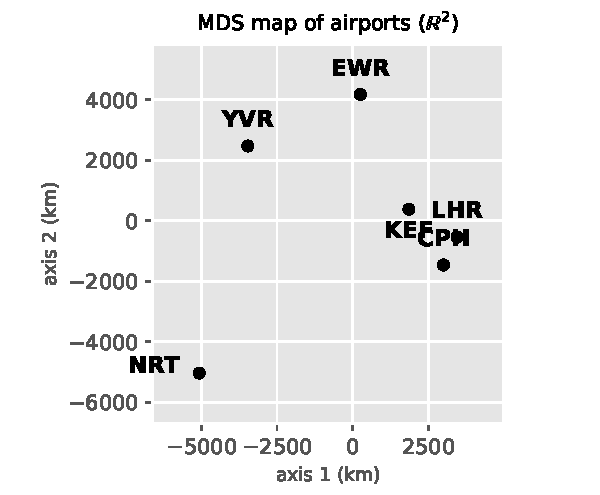
\includegraphics[width=0.56\textwidth]{fig_q2_map.pdf}
  \caption{MDS embedding of the six airports in $\mathbb{R}^2$. The relative layout is consistent with real geography up to an arbitrary rotation/reflection: the European cluster CPH--KEF--LHR sits together (with KEF reaching towards the Atlantic), EWR lies across the Atlantic, YVR is on the Pacific side of North America, and NRT (Tokyo) is the most isolated point.}
  \label{fig:q2map}
\end{figure}

\subsection{Part (b) --- accuracy of the map}

We report the raw stress $S_M$ and the scale-free \emph{Kruskal stress-1},
$\text{stress-1}=\sqrt{S_M/\sum_{i<j}d_{ij}^2}$,
and draw a Shepard diagram comparing embedded distances to true distances.

\begin{lstlisting}
iu = np.triu_indices(n, 1)
d_true = D[iu];  d_map = pairwise_distances(Z)[iu]
kruskal = np.sqrt(mds2.stress_ / np.sum(d_true ** 2))
print("S_M = %.4e km^2,  Kruskal stress-1 = %.4f (%.2f%%)"
      % (mds2.stress_, kruskal, 100 * kruskal))
# S_M = 1.5086e+05 km^2,  Kruskal stress-1 = 0.0149 (1.49%)

lim = d_true.max() * 1.07
plt.figure(figsize=(3.5, 3.5))
plt.plot([0, lim], [0, lim], "k-", lw=1)
plt.scatter(d_true, d_map, color="salmon", edgecolor="k")
plt.xlabel("true distance (km)");  plt.ylabel("map distance (km)")
plt.title("Shepard diagram");  plt.tight_layout();  plt.show()
\end{lstlisting}

The Kruskal stress-1 is $1.49\%$ and the largest pairwise error is $194$\,km (against distances up to $10\,833$\,km), confirming the map is accurate in relative terms. It \textbf{cannot be perfectly accurate} because the given values are \emph{great-circle (geodesic) distances on the sphere} $\mathbb{S}^2$. As the Week~4 slides illustrate ($\mathbb{S}^2\to\mathbb{R}^2$), a curved 2-manifold cannot be flattened into the Euclidean plane without distorting distances, so MDS's flat proxy always leaves a non-zero stress.

\subsection{Part (c) --- embedding in \texorpdfstring{$\mathbb{R}^d$}{Rd} for \texorpdfstring{$d>2$}{d>2}}

We repeat MDS for $d=1,\dots,5$ (with $n=6$ points, at most $n-1=5$ dimensions are useful) with identical settings and plot the minimised stress.

\begin{lstlisting}
dims = list(range(1, 6));  stresses = []
for d in dims:
    m = MDS(n_components=d, dissimilarity="precomputed", random_state=1234,
            normalized_stress=False, init="random", n_init=300,
            max_iter=1000, eps=1e-10)
    m.fit_transform(D);  stresses.append(m.stress_)
plt.figure(figsize=(4, 2.8))
plt.plot(dims, stresses, "-o", color="royalblue");  plt.xticks(dims)
plt.xlabel("dimension d");  plt.ylabel("stress S_M (km^2)")
plt.title("Stress vs. embedding dimension");  plt.tight_layout();  plt.show()
# d=1: 4.54e7,  d=2: 1.51e5,  d=3: 1.45e5,  d=4,5: 1.45e5 (plateau)
\end{lstlisting}

\begin{figure}[H]
  \centering
  \begin{minipage}[t]{0.46\textwidth}
    \centering
    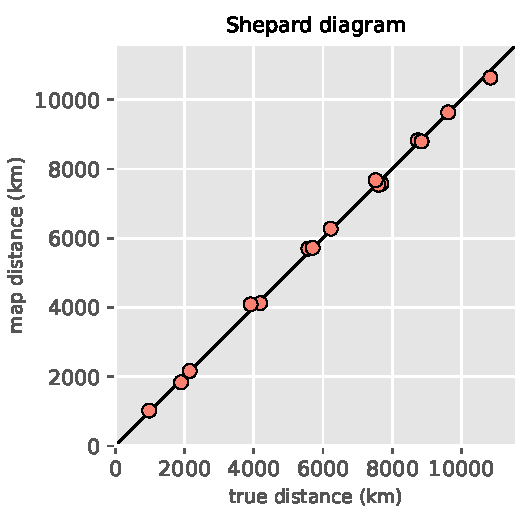
\includegraphics[width=\textwidth]{fig_q2_shepard.pdf}
    \caption{Shepard diagram for the $\mathbb{R}^2$ map. Points lie close to the diagonal, confirming a good relative fit.}
    \label{fig:shepard}
  \end{minipage}\hfill
  \begin{minipage}[t]{0.50\textwidth}
    \centering
    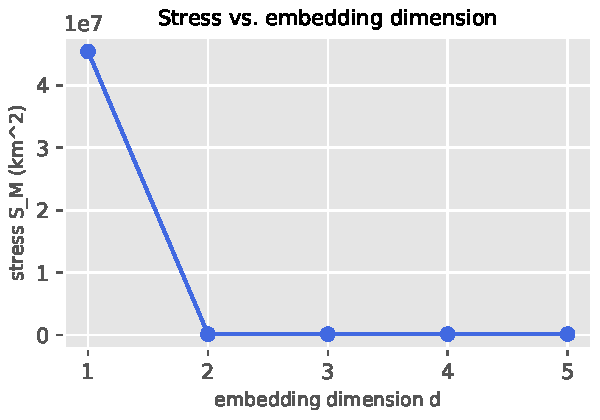
\includegraphics[width=\textwidth]{fig_q2_stress.pdf}
    \caption{Minimum stress $S_M$ vs.\ embedding dimension $d$. Stress falls sharply from $d=1$ to $d=2$, improves slightly at $d=3$, then plateaus and stays strictly positive.}
    \label{fig:stress}
  \end{minipage}
\end{figure}

\subsection{Conclusion}

Increasing $d$ adds degrees of freedom, so the minimum stress is \textbf{non-increasing} in $d$ and accuracy improves --- from $d=1$ (stress $4.54\times10^7$) to $d=2$ ($1.51\times10^5$, Kruskal $1.49\%$) to $d=3$ ($1.45\times10^5$), after which it \textbf{plateaus}: $d=4$ and $d=5$ give essentially the same stress as $d=3$. The plateau reflects the intrinsic geometry: the airports lie on the 2-sphere, so three Euclidean dimensions already capture essentially all the embeddable structure.

Crucially, the stress \textbf{never reaches zero}, even at $d=5$. Great-circle distances on a sphere are \emph{not} Euclidean distances in any dimension; no finite-dimensional Euclidean embedding can be exact and a non-zero irreducible stress always remains. The practical gain beyond $\mathbb{R}^2$ is small, so the 2-D map of Part~(a) is already a faithful relative representation.

% ============================================================
\section{PCA cannot, but ICA can, recover mixed sources}

\subsection{Problem and construction rationale}

We build three one-dimensional signals $x_1,x_2,x_3$ (sine, square, sawtooth), form mixtures
$Y=AX$ via a fixed $3\times3$ matrix $A$, and ask whether PCA or ICA can recover $X$ from $Y$ alone.

Two design choices make the contrast sharp. \textbf{(1) Non-Gaussian, independent sources.}
ICA assumes at most one Gaussian source; rotating independent Gaussians produces independent
Gaussians again, so a purely Gaussian model is unidentifiable. Our three waveforms---sine (arcsine
distribution), square (bimodal), sawtooth (uniform)---are manifestly non-Gaussian and
independent. \textbf{(2) Non-orthogonal} $A$. PCA finds orthogonal variance directions. If $A$ is
not orthogonal, the true source directions in observation space are not orthogonal and PCA's axes
cannot align with them---the principal components remain mixtures. ICA fixes the rotation PCA
leaves undetermined by maximising statistical independence (higher-order statistics), recovering
the sources up to the known caveats of order, sign, and scale.

\begin{lstlisting}
import numpy as np, matplotlib.pyplot as plt
from scipy import signal
from scipy.optimize import linear_sum_assignment
from sklearn.decomposition import PCA, FastICA

rng = np.random.default_rng(0)
n = 2000;  t = np.linspace(0, 8, n)
x1 = np.sin(2 * t)                      # sine
x2 = np.sign(np.sin(3 * t))             # square
x3 = signal.sawtooth(2 * np.pi * t)     # sawtooth
X = np.vstack([x1, x2, x3])
X = X + 0.02 * rng.standard_normal(X.shape)
X = (X - X.mean(axis=1, keepdims=True)) / X.std(axis=1, keepdims=True)

A = np.array([[1.0, 1.0, 1.0],
              [0.5, 2.0, 1.0],
              [1.5, 1.0, 2.0]])          # non-orthogonal: A @ A.T != c*I
Y = A @ X
\end{lstlisting}

\subsection{PCA on the mixtures (fails)}

\begin{lstlisting}
pca = PCA(n_components=3)
Z = pca.fit_transform(Y.T)
Z = (Z / np.max(np.abs(Z), axis=0)).T   # normalise scale; back to 3 x n

def corr_matrix(R, S):
    M = np.zeros((R.shape[0], S.shape[0]))
    for i in range(R.shape[0]):
        for j in range(S.shape[0]):
            M[i, j] = np.abs(np.corrcoef(R[i], S[j])[0, 1])
    return M

C_pca = corr_matrix(Z, X)
# |corr| matrix (rows = PC1-3, cols = x1,x2,x3):
# [[0.516 0.612 0.601]
#  [0.407 0.782 0.437]
#  [0.753 0.119 0.670]]
\end{lstlisting}

No principal component is strongly aligned with a single source: every row mixes substantial
correlation across several sources and no clean one-to-one matching exists. The best
$|\text{corr}|$ each PC achieves with any source is $0.61,\,0.78,\,0.75$---all well below $1$.
This is expected: PCA can only decorrelate and must return \emph{orthogonal} components, but
the columns of $A$ are not orthogonal, so its axes cannot recover the source directions.

\subsection{ICA on the mixtures (succeeds)}

\begin{lstlisting}
ica = FastICA(n_components=3, whiten="unit-variance", random_state=0, max_iter=1000)
S = ica.fit_transform(Y.T)
S = (S / np.max(np.abs(S), axis=0)).T

C_ica = corr_matrix(S, X)
# |corr| matrix (rows = IC1-3, cols = x1,x2,x3):
# [[0.997 0.030 0.069]
#  [0.055 0.015 0.997]
#  [0.058 0.999 0.037]]
row, col = linear_sum_assignment(-C_ica)
order = col[np.argsort(row)]
matched = C_ica[np.arange(3), order]   # [0.9968, 0.9969, 0.9994]
\end{lstlisting}

Each IC has $|\text{corr}|\approx 1$ with exactly one source and $\approx 0$ with the other two.
The optimal assignment maps IC1$\to x_1$, IC2$\to x_3$, IC3$\to x_2$, with matched
$|\text{corr}|=0.997,\,0.997,\,0.999$ and maximum recovery error $1-|\text{corr}|=0.003$.

\begin{figure}[H]
  \centering
  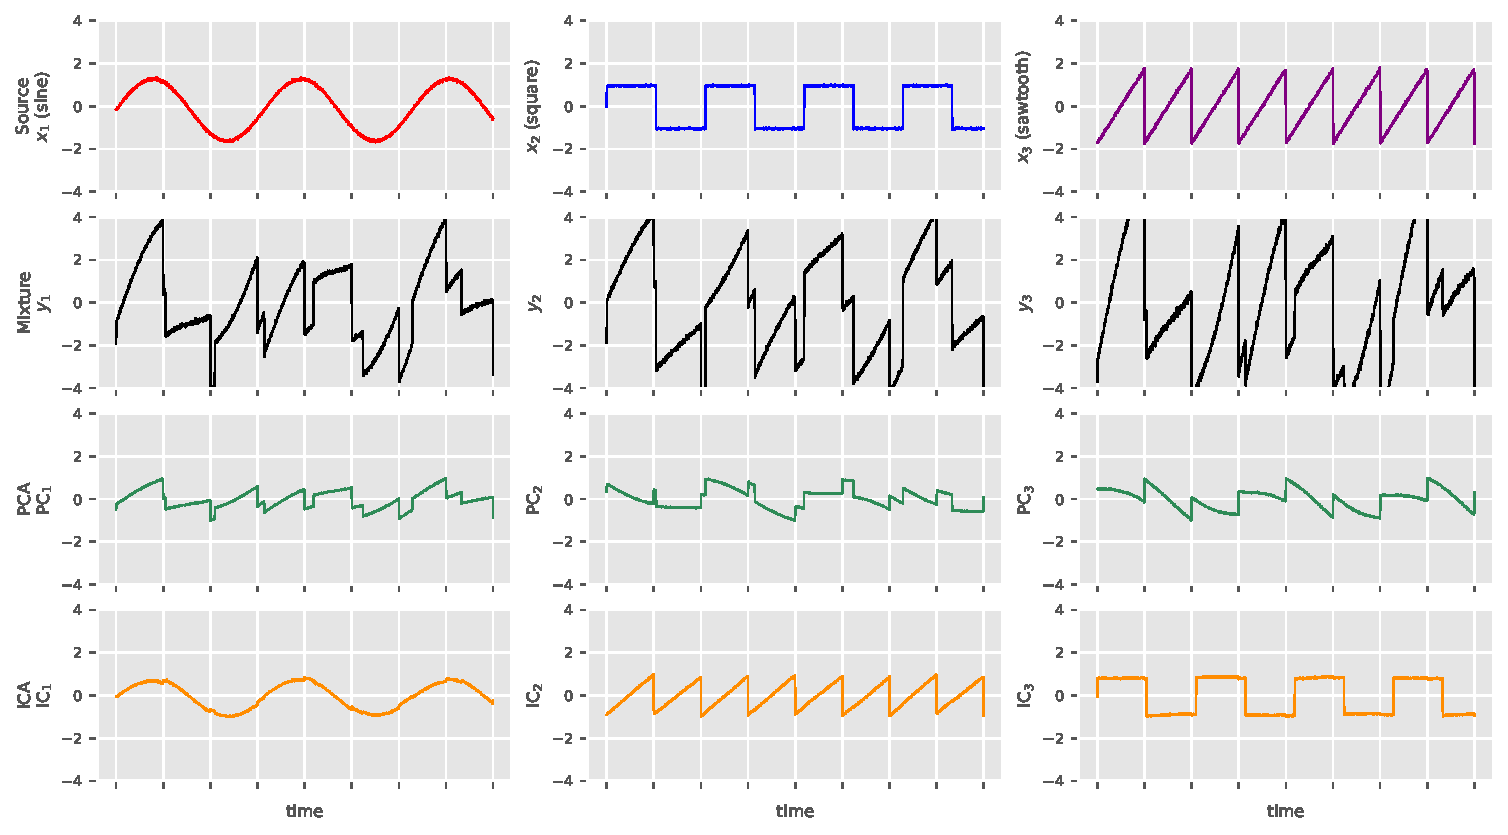
\includegraphics[width=0.97\textwidth]{fig_q3_rows.pdf}
  \caption{Row 1: original sources; Row 2: observed mixtures $Y=AX$; Row 3: principal components
  (still mixed); Row 4: independent components (source shapes restored).}
  \label{fig:q3rows}
\end{figure}

\begin{figure}[H]
  \centering
  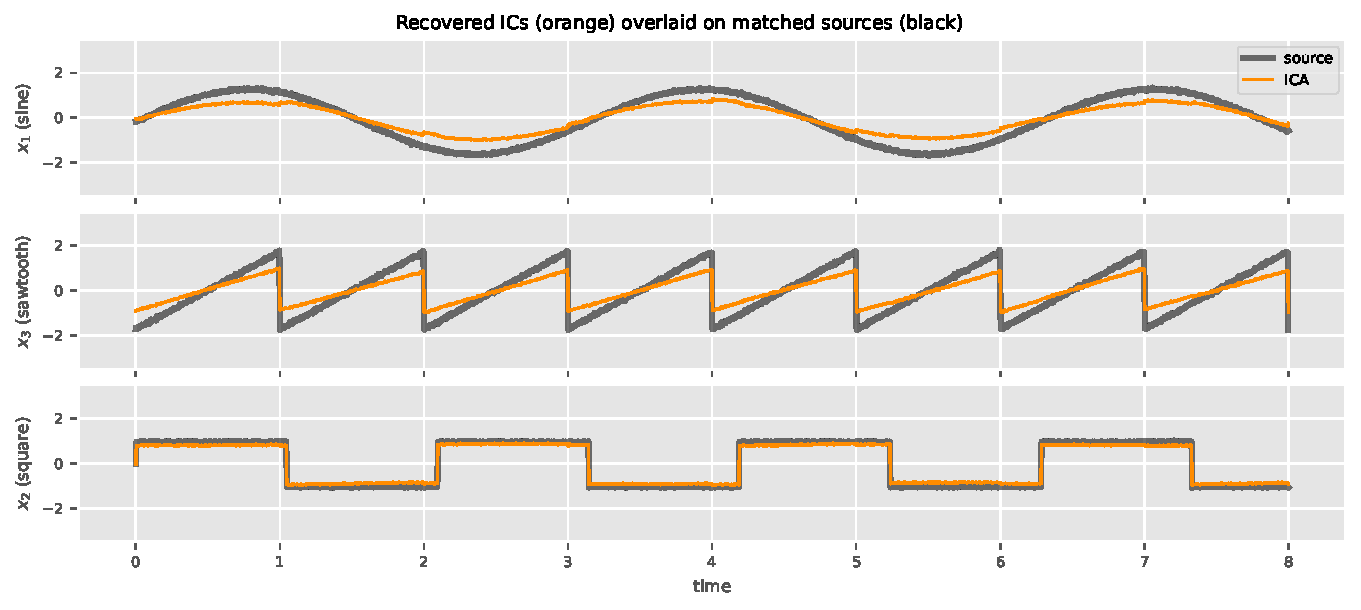
\includegraphics[width=0.87\textwidth]{fig_q3_overlay.pdf}
  \caption{ICA recovery: each independent component (orange) overlaid on its matched source (black).
  The waveforms are virtually indistinguishable, confirming $|\text{corr}|\approx 1$.}
  \label{fig:q3overlay}
\end{figure}

\subsection{Conclusion}

\begin{table}[h]
  \centering\small
  \begin{tabular}{llll}
    \toprule
    Method & Criterion & Best $|\text{corr}|$ & Recovers sources? \\
    \midrule
    PCA  & orthogonal max-variance directions (2nd-order) & $0.61,\,0.78,\,0.75$ & \textbf{No}  \\
    ICA  & statistical independence / non-Gaussianity     & $1.00,\,1.00,\,1.00$ & \textbf{Yes} \\
    \bottomrule
  \end{tabular}
  \caption{PCA vs.\ ICA on the cocktail-party problem.}
\end{table}

PCA leaves a rotation of the whitened space undetermined---that rotation is invisible to
second-order statistics. Since $A$ is not orthogonal, the source axes are not orthogonal, so
PCA's axes cannot coincide with them and the principal components remain mixed. ICA resolves the
undetermined rotation by demanding maximally independent/non-Gaussian components; because at most
one source is Gaussian, this uniquely identifies the sources up to the unavoidable permutation,
sign, and scale ambiguity---confirmed empirically by $|\text{corr}|\approx 1$.

% ============================================================
\section{Distance Concentration and the Curse of Dimensionality}

\subsection{Problem and simulation}

We study how the ratio
\[
  R := \frac{\max_{i\neq j}\lVert X_i-X_j\rVert}{\min_{i\neq j}\lVert X_i-X_j\rVert},
  \qquad X_1,\dots,X_{10}\overset{\text{i.i.d.}}{\sim}N_d(0,I_d),
\]
behaves as $d\to\infty$, averaged over 200 independent realisations per $d$.

\begin{lstlisting}
import numpy as np, matplotlib.pyplot as plt
from scipy.spatial.distance import pdist

rng = np.random.default_rng(42)
d_values = [2, 5, 10, 50, 100, 500, 1_000, 5_000, 10_000, 50_000, 100_000]
n_rep, n_pts = 200, 10

R_means, R_stds = [], []
for d in d_values:
    ratios = [pdist(rng.standard_normal((n_pts, d))).max()
              / pdist(rng.standard_normal((n_pts, d))).min()
              for _ in range(n_rep)]
    R_means.append(np.mean(ratios)); R_stds.append(np.std(ratios))
\end{lstlisting}

\begin{figure}[H]
  \centering
  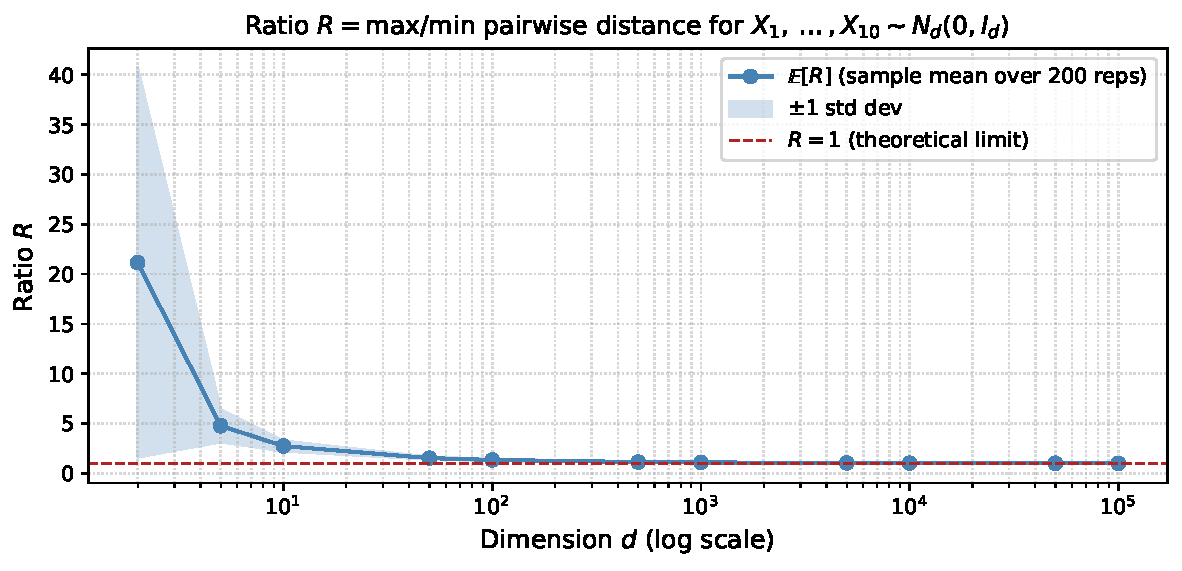
\includegraphics[width=0.82\textwidth]{fig_q4_ratio.pdf}
  \caption{Mean $\pm1$ std of $R$ over 200 repetitions as a function of $d$ (log scale).
  $R\to 1$ rapidly; standard deviation also collapses, showing tight concentration.}
  \label{fig:q4ratio}
\end{figure}

\subsection{Theoretical explanation (LLN and CLT)}

Fix any pair $(i,j)$. Since $X_{i,k},X_{j,k}\overset{\text{i.i.d.}}{\sim}N(0,1)$, the
differences $Z_k:=X_{i,k}-X_{j,k}\sim N(0,2)$, giving
\[
  \|X_i-X_j\|^2 = \sum_{k=1}^d Z_k^2,\quad
  \mathbb{E}[Z_k^2]=2,\quad \operatorname{Var}(Z_k^2)=8.
\]
By the \textbf{Law of Large Numbers}
\[
  \frac{\|X_i-X_j\|^2}{2d}\xrightarrow{p}1
  \;\Longrightarrow\;
  \frac{\|X_i-X_j\|}{\sqrt{2d}}\xrightarrow{p}1 \quad\text{as }d\to\infty.
\]
The \textbf{CLT} gives the rate: $\bigl(\|X_i-X_j\|^2-2d\bigr)/\sqrt{8d}\to N(0,1)$,
so fluctuations around $\sqrt{2d}$ are of order $d^{-1/2}\to 0$.

There are only $\binom{10}{2}=45$ pairs---a fixed finite number independent of $d$. By a
union bound, \emph{all} 45 distances concentrate around the same value $\sqrt{2d}$
simultaneously, so the maximum and minimum converge to the same limit and
\[
  R = \frac{\max_{i\neq j}\|X_i-X_j\|}{\min_{i\neq j}\|X_i-X_j\|}\xrightarrow{p}1
  \qquad\text{as }d\to\infty.
\]
The histograms below (200 repetitions, all 45 distances per repetition, normalised by
$\sqrt{2d}$) confirm the increasing concentration around~1.

\begin{lstlisting}
d_check = [10, 100, 1_000, 10_000];  n_rep2 = 500
for d in d_check:
    all_norm = [v for _ in range(n_rep2)
                for v in (pdist(rng.standard_normal((n_pts, d))) / np.sqrt(2 * d)).tolist()]
    # histogram of all_norm concentrates at 1 as d grows
\end{lstlisting}

\begin{figure}[H]
  \centering
  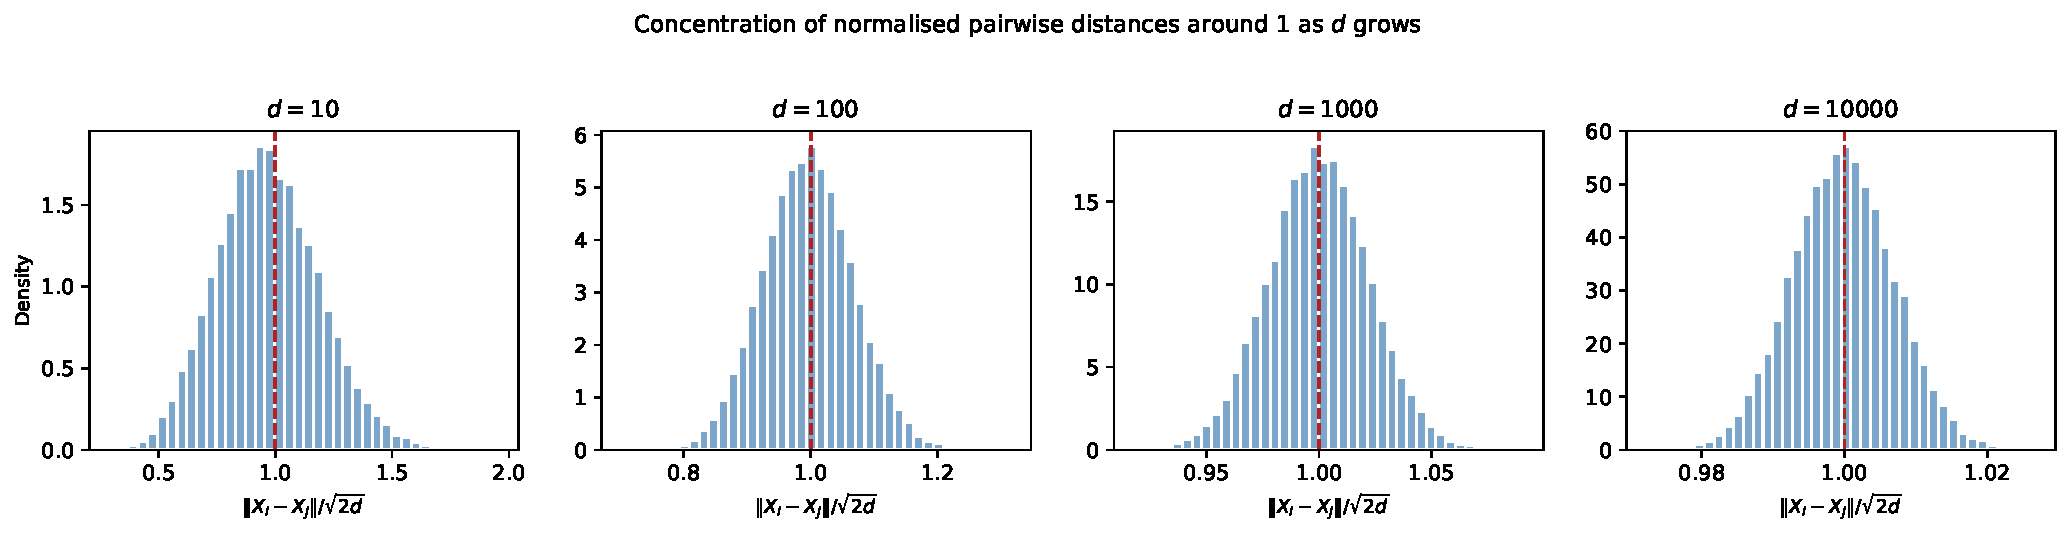
\includegraphics[width=0.97\textwidth]{fig_q4_concentration.pdf}
  \caption{Histograms of $\lVert X_i-X_j\rVert/\sqrt{2d}$ over 500 repetitions $\times$ 45 pairs
  at four values of $d$. The distribution tightens around 1, with variance $O(1/d)$ as predicted.}
  \label{fig:q4conc}
\end{figure}

\subsection{Relation to the curse of dimensionality}

When $R\approx 1$, every pair of points is roughly equidistant---the concept of a
\emph{nearest neighbour} becomes meaningless because ``near'' and ``far'' are indistinguishable.
This breaks many unsupervised learning algorithms.

\begin{itemize}[noitemsep,topsep=2pt]
  \setlength\itemsep{1pt}
  \item \textbf{$K$-means / $K$-medoids (Week~3).} Cluster assignment picks the closest centroid.
        If all distances are nearly equal, every point is equidistant from all centroids and
        assignments become essentially arbitrary.
  \item \textbf{MDS (Week~4).} MDS preserves pairwise distances. When all distances concentrate
        at $\sqrt{2d}$, the data look like points on a sphere and a meaningful low-dimensional
        embedding ceases to exist.
\end{itemize}

This is the key motivation for dimensionality reduction \emph{before} applying distance-based
methods: techniques such as PCA (Weeks~2--3) and ICA (Week~2) project the data onto a
lower-dimensional subspace where distances remain informative and $R$ is bounded away from~1.

\end{document}
